%
\documentclass[Proceedings]{ascelike}
%
% Feb. 14, 2013
%
% Some useful packages...
%
\usepackage{graphicx}
%\usepackage{subfigure}
\usepackage{amsmath}
%\usepackage{amsfonts}
%\usepackage{amssymb}
%\usepackage{amsbsy}
%\usepackage{times}
%
%
% Place hyperlinks within the pdf file (works only with pdflatex, not latex)
% \usepackage[colorlinks=true,citecolor=red,linkcolor=black]{hyperref}
%
%
% NOTE: Don't include the \NameTag{<your name>} if you have selected 
%       the NoPageNumbers option: this leads to an inconsistency and
%       a warning, and the NameTag is ignored.
%\NameTag{Kuhn, Feb. 14, 2013}
%
%
\begin{document}
%
% You will need to make the title all-caps
\title{Determinaci\'on del periodo de la orbita de una estrella binaria espectrosc\'opica.}
%
\author{
Nicolas Garavito-Camargo,%
%
% ---- The first of two styles for addresses: using footnotes and \thanks ----
\thanks{
Dept.\ de F\'isica.,
Universidad de los Andes, 
Calle 1...\ Bogot\'a, Colombia. E-mail: jn.garavito57@uniandes.edu.co}
\ Benjamin Oostra\footnotemark[1]
%
% Adding a second author with the same affiliation (still using \thanks):
%  \\
 %Colleague,\footnotemark[1] Member, ASCE%
%
% Adding another author with a different affiliation.  I have found that 
% the \and command doesn't quite work, so just use "and", as in the following 
% \\
% and
% Younyee Kuhn%
% \thanks{Flourishing wife of same.},%
% \ Not a Member, ASCE
%
% ---- The second of two styles for addresses: below names, no footnotes ----
%
% For this style, don't use \thanks.  Instead, use superscripts and carriage
% returns ("\\").  It's not pretty, but neither is the new ASCE proceedings
% style.  Something like the following:
%
% Matthew R. Kuhn$^1$, Member, ASCE\\[1ex]%
%
% $^1$\parbox[t]{5.75in}{Dept.\ of Civil Engrg.,
% Donald P.\ Shiley School of Engrg., Univ.\ of Portland, 
% 5000 N.\ Willamette Blvd., Portland, OR  97203. kuhn@up.edu.}
}
%
\maketitle
%

\section*{Introducci\'on}

En astronom\'ia a diferencia de la f\'isica no se pueden realizar experimentos ya
que solo hay un universo observable. Por lo tanto de este se tiene que obtener 
toda la informaci\'on posible por medio de observaciones y con estas poder entender 
los fen\'onemos f\'isicos presentes en el universo.

A partir de estas observaciones en particular de la espectroscop\'ia se obtiene informaci\'on,
sobre la abundancia de elementos quimicos, las velocidades radiales, tasas de formacion estelar, 
masas de estrellas etc.

Estas observaciones son de la radiaci\'on proveniente del universo y se hacen
 en diferentes longitudes de onda del espectro electromagnetico. Estas longitudes 
 de onda se dividen en: Microondas, Rayos X, Infrarojo, Visible, Radio, UV. La observaci\'on 
 en estas frecuencias depende en gran medida de las ventanas presentes en la atmosfera terrestre.
Las principales ventanas se encuentran en el rango visible y en ondas de radio por lo que muchos telescopios terrestres son de este tipo. 

El objetivo de este trabajo es familiarizarse con las tecnicas observacionales en astronomia en particular
con el uso de espectros astron\'omicos, para esto se pretende observar una estrella binaria $\varepsilon$ CRA 
y encontrar su periodo orbital a partir de la medici\'on de su espectro. Este estudio por medio de espectros es muy utilizado en astronomia y estudiar estrellas binarias es de gran importancia ya que se estima que el $50\%$ de estrellas en la via l\'actea son binarias.  

Por otro lado conociendo la orbita de estrellas es posible reconstruir el potencial gravitacional 
del sistema, lo cual es de bastante utilidad ya que muchas veces el potencial gravitacional no es conocido para sistemas complejos (Via l\'actea). reconstruir el potencial gravitacional del sistema binario se deja como 
complemento de este trabajo.\\
\\

\section{Marco Te\'orico}

\subsection{Espectrografia}

La espectrografia es una tecninca en la cual la luz se descompone en las diferentes
longitudes de onda. A partir de la intensidad de las diferentes lineas de emisi\'on/absorci\'on
se pueden encontrar cantidades f\'isicas, tales 
como la composici\'on quimica, temperatura superficial, la masa, tasas de formacion estelar
 y si hay presencia de medio interestelar se puede hallar la cinem\'atica del gas. [2]
 
Conociendo los espectros estelares es posible reconstruir sint\'eticamente espectros de galaxias
y asi saber las poblaciones estelares presentes en cada galaxia y si se hace esto para galaxias
con diferentes edades es posible ver como evolucionan las poblaciones estelares en las galaxias 
con el tiempo.

La espectrografia es la tecnica mediante la cual se puede obtener mas informaci\'on de la radiacion 
proveniente de los diferentes objetos celestes.

\subsection{Clasificacion espectral de las estrellas}

Esta clasificaci\'on de denomina clasificaci\'on espectral de Harvard en esta las estrellas se clasifican seg\'un su temperatura as\'i:[2]\\

O-B-A-F-G-K-M-L-T\\

\begin{itemize}

\item O son estrellas de azules (calientes) de temperatura superficial entre 20000K y 35000K.\\
\item B son estrellas azules-blancas de temperatura superficial de 15000K.\\
\item A son estrellas blancas de temperatura superficial de 9000K.\\
\item F son estrellas blancas-amarillas con temperatura superficial de 7000K.\\
\item G son estrellas amarillas como nuestro sol con temperatura superficial de 5500K.\\
\item K son estrellas naranjas-amarillas con una temperatura superficial de 4000K.\\
\item M son estrellas rojas de temperatura superficial de 3000K.\\
\item L son estrellas marronas con temperatura superficial de 2000K.\\
\item T son enanas marrones con temperatura superfical de 1000K.\\
\end{itemize}


\subsection{Binarias espectrosc\'opicas}

Las estrellas binarias espectrosc\'opicas solo se pueden detectar mediante sus espectros,  
estos espectros muestran dos veces las lineas de absorci\\on o emisi\'on una con corrimiento hacia 
el rojo y la otra al azul debido al movimiento [poner referencia a nuestro espectro]
orbital de las estrellas, donde la maxima separacion sera cuando una estrella se aleja de la
linea de vision y la otra se acerca, el periodo de estas separaciones correspondera al periodo
orbital de la binaria.

Para encontrar la velocidad relativa tenemos que:
\begin{equation}
\dfrac{v}{c} \simeq z = \dfrac{\lambda_{o} - \lambda_{e}}{ \lambda_{e}}
\end{equation} 

\section{Seleci\'on de la binaria a observar}

Para la seleci\'on de la estrella binaria a observar se tuvieron en cuenta 
diferentes caracteristicas tales como:

\begin{itemize}
\item Visibilidad en nuestra ubicacion, (AR $> 16$h, Declinacion $(-40^{0}, 80^{0})$)
\item Magnitud aparante menor a 5, (M $<5$).
\item La duraci\'on del periodo menor a 2 meses.
\item Estrellas calientes para obtener mas lineas de emision y as\'i poder
encontrar la oribta con mayor exactitud.
\end{itemize}

Despues de tener en cuenta los parametros en el cat\'alogo de estrellas binarias [3] encontramos los siguientes candidatos:\\

\begin{tabular}{c c c c c c}
\hline
Nombre & RA & DEC & Periodo (D\'ias) & Tipo espectral & Magnitud\\
\hline
$\varepsilon$ $\mathrm{CRA}$ & 18h59m39s & $-37^{0}05' 17''$ & 0.59 & F0V & 4.8\\
\hline
$\mu 1$ $\mathrm{Sco}$ & 16h52m48s & $-38^{0}04'11''$& 1.44 & B1.5V& 3.00\\
\hline
\\
\end{tabular}
\\
Entre estas dos estrellas se selecciono Epsilon de la Coronae Australis (${\epsilon}$ CRA) ubicada en la 
constelacion de la Coronae Australis Fig. \ref{la}, ya que su periodo es el mas corto, pero tambien se tomaron 
espectros de $\mu 1$ del escorpion. 


\begin{figure}
\centering
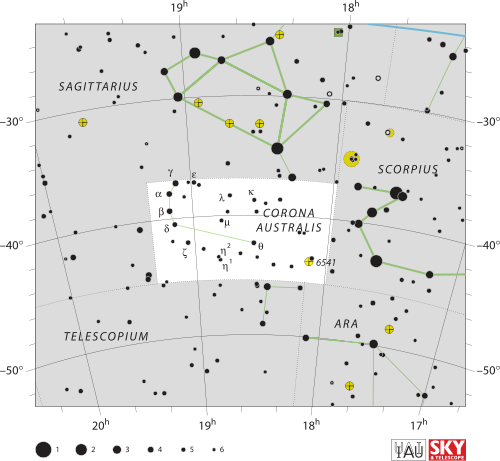
\includegraphics[scale=0.4]{CRA.png}
\caption{Corona Australis [5]\label{la}}
\end{figure}


\section{Observaciones}

Todas las observaciones se han llevado acabo en el observatorio astronomico de la 
Universidad de los Andes. A continuaci\'on se describen la instrumentacion utlizada
as\'i como los protocolos de observaci\'on utilizados.

El montaje experimental que se utilizo se muestra en la Fig. \ref{montaje} en el cual se ve el acople
de las fibras \'opticas al telescopio, por medio de estas fibras las luz es llevada hasta
el espectr\'ografo.

\subsection{Instrumentaci\'on}

\subsubsection{Telescopio}

Se utiliz\'o un telescopio marca Meade LX200 Schimdt-Cassegrain Fig.\ref{la} de $40 cm$ de apertura y una
distancia focal de $4m$.

\begin{figure}
\centering
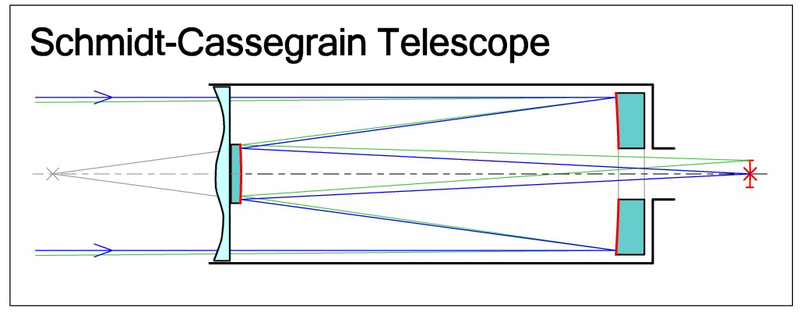
\includegraphics[scale=0.4]{SCT2.jpg}
\caption{Camino de luz en un telescopio Schmidt-Cassegrain [6] \label{la}}
\end{figure}


\subsubsection{Espectrografo}

El espectr\'rografo que se utilizo (Espartaco) Fig.\ref{espectrografo} es un espectrografo de alta resolucion en el cual la luz del telescopio llega por medio de una fibra \'optica, luego esta luz es descompuesta por una rendija de difracci\'on y finalmente la radiaci\'on es recolectada en una CCD.


\begin{figure}
\centering
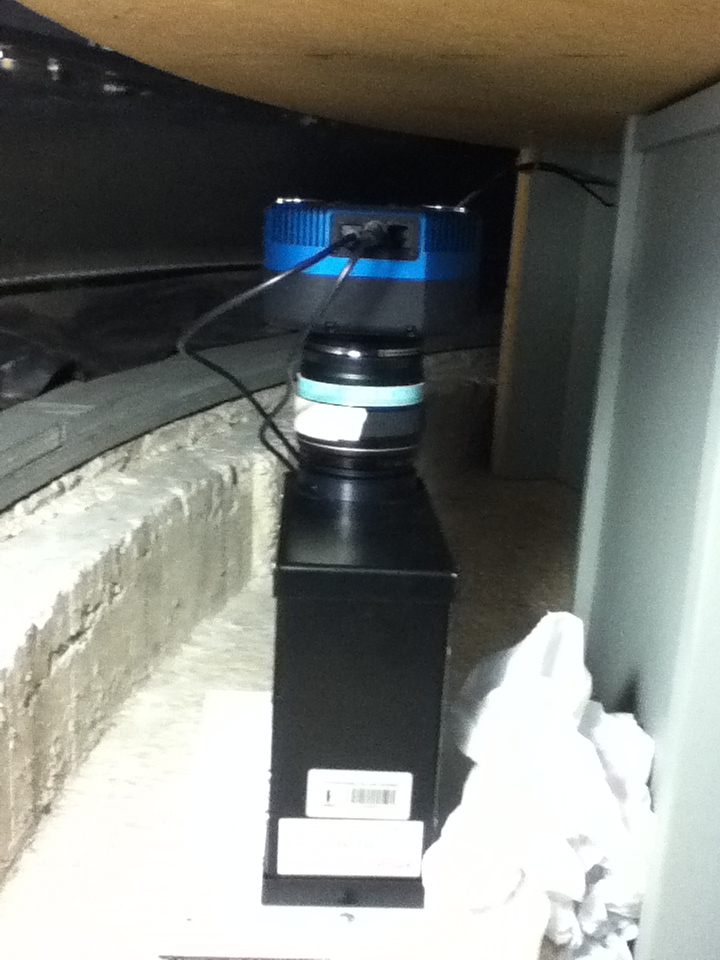
\includegraphics[scale=0.2]{espectroscopio.jpg}
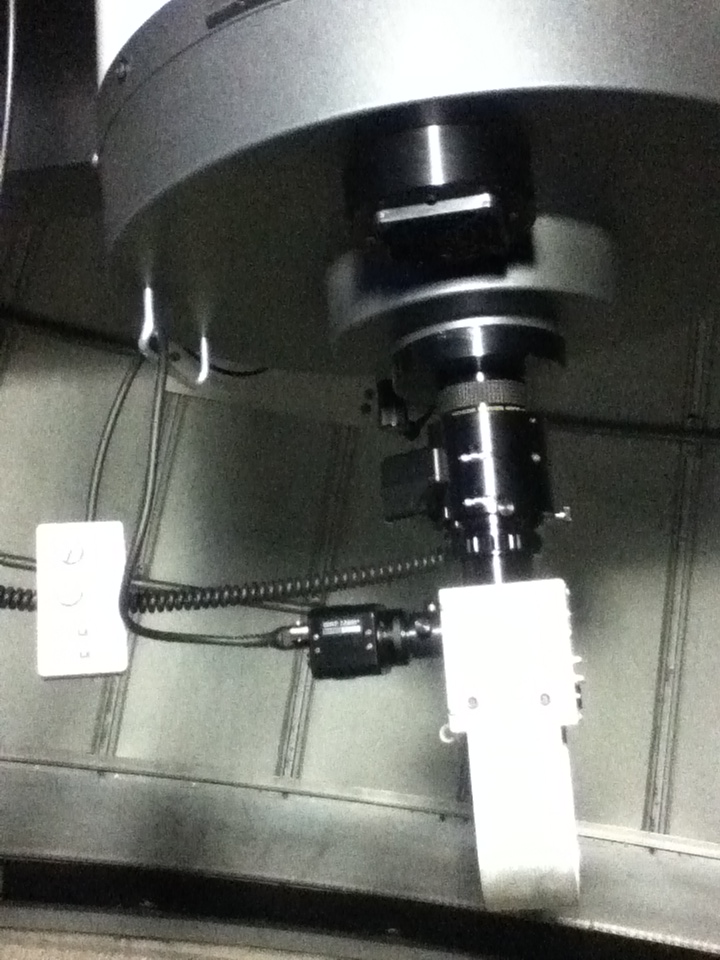
\includegraphics[scale=0.2]{montaje.jpg}

\caption{Espectrografo (Izquierda), Montaje experimental (Derecha) \label{espectrografo}}
\end{figure}



\subsubsection{Software}

La reducci\'on de datos se llevo acabo con el software ISIS [4]
el cual usa como referencia los espectros de las lamparas de calibracion (de torio y tungsteno)
para obtener los perfiles de los espectros tomados de las estrellas.

\subsection{Protocolo de Observacion}

Todas las observaciones se han llevado acabo en el observatorio de astronomico
de la universidad de los andes. Los datos ac\'a presentados se tomaron las noches
del 10, 13 y 16 de septiembre de 2013. En un intervalo de tiempo aproximadamente 
desde las 5pm hasta las 10 pm. 

El protocolo de observacion que se sigio fue el siguiente:

\begin{itemize}
\item Preparar el montaje, conectar el espectroscopio al telescopio haciendo de las 
fibras opticas.
\item Tomar espectros de las lamparas de calibraci\'on 
\item Posicionar la fibra optica en el foco del telescopio
\item Encontrar la estrella binaria $\varepsilon CRA$ y enfocarla en la fibra optica
\item Tomar los espectros, entre 5 y 15 min cada uno.
\end{itemize}

\section{Resultados preliminares}

A continuaci\'on Fig. \ref{eps} se muestran 3 espectros que se tomaron en 3 diferentes dias, cada uno de 
estos espectros representa la mejor medicion del dia en que se tomaron. Todos los espectros
tomados se encuentran a disposicion en el repositorio https://github.com/jngaravitoc/EpsCra/tree/master/data.
Es importante resaltar que se han tomado muchos mas espectros pero se han tenido problemas con la contaminacion 
luminica, nubosidad y un error en el monataje experimental que hizo que los espectros resultantes no fueran 
apropiadas para el estudio que se pretende realizar.

\begin{figure}
\centering
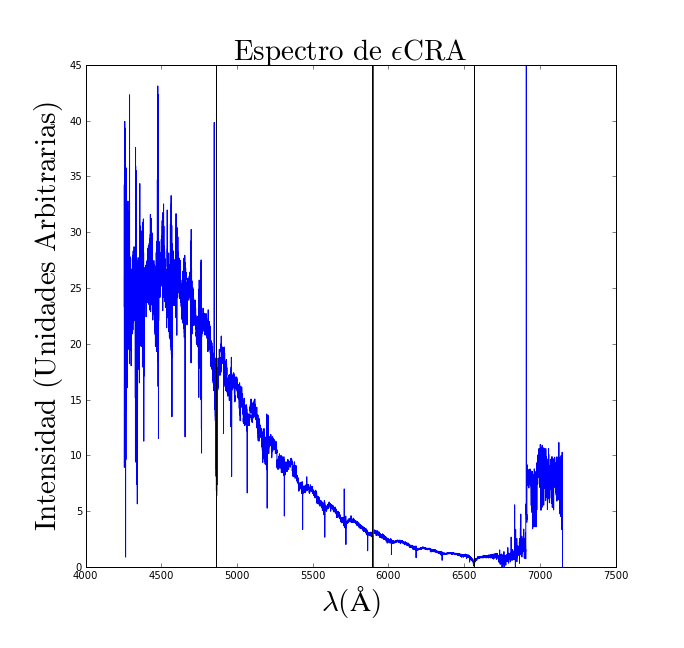
\includegraphics[scale=0.33]{Espectro1.png}
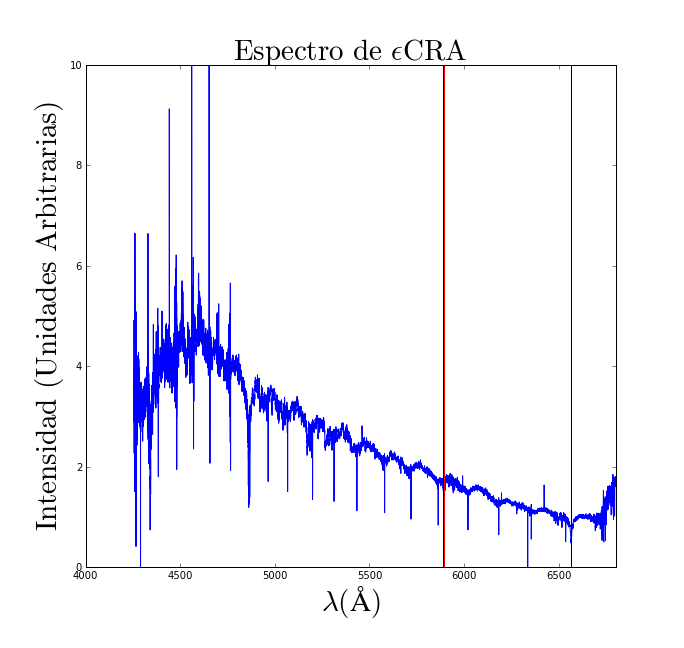
\includegraphics[scale=0.33]{Espectro2.png}
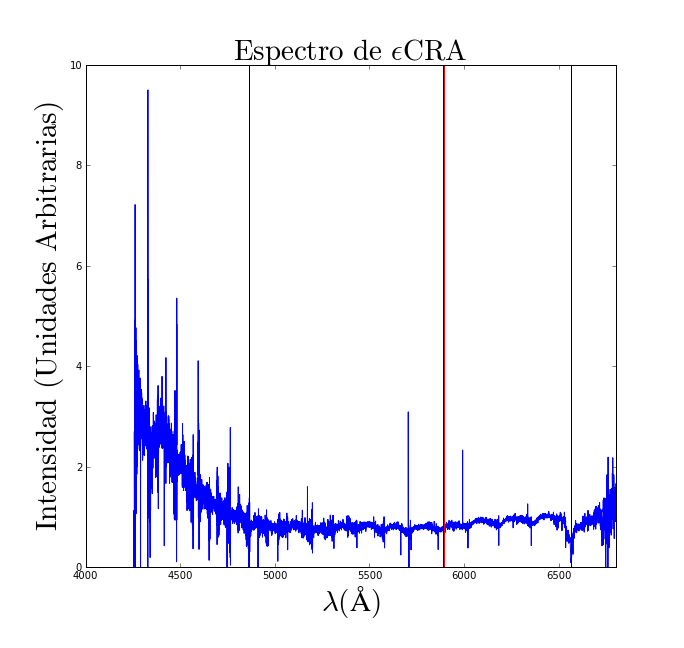
\includegraphics[scale=0.33]{Espectro3.png}
\caption{Tres diferentes espectros de eps CRA\label{eps}}
\end{figure}

A partir de la Fig. \ref{eps} se pueden buscar las principales lineas de absorci\'on como por ejemplo $H\alpha$
Fig. \ref{ha} y con esta hallar informaci\'on sobre el periodo de la estrella binaria. Pero debido a los pocos espectros obtenidos hasta el momento no es posible encontrar el periodo de la orbita. Lo que es posible hallar es la velocidad a la cual el sistema se esta alejando de nosotros haciendo uso de la ecuaci\'on (1) y (2).\\

\begin{tabular}{c c c c}
\hline
Espectro & Velocidad ($km/s$) & $v_{teo}$ ($km/s$) [3]& Error \%  \\
\hline
1 & 63.69 & 61.9 & 2.89\\
2 & 63.69 & 61.9 & 2.89 \\
3 & 63.69 & 61.9 & 2.89\\
\hline
\end{tabular}

\begin{figure}
\centering
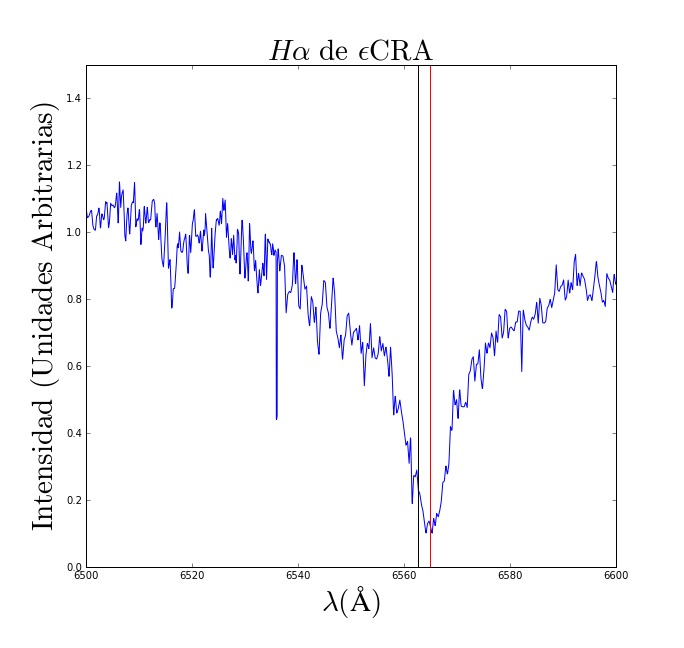
\includegraphics[scale=0.33]{ha1.png}
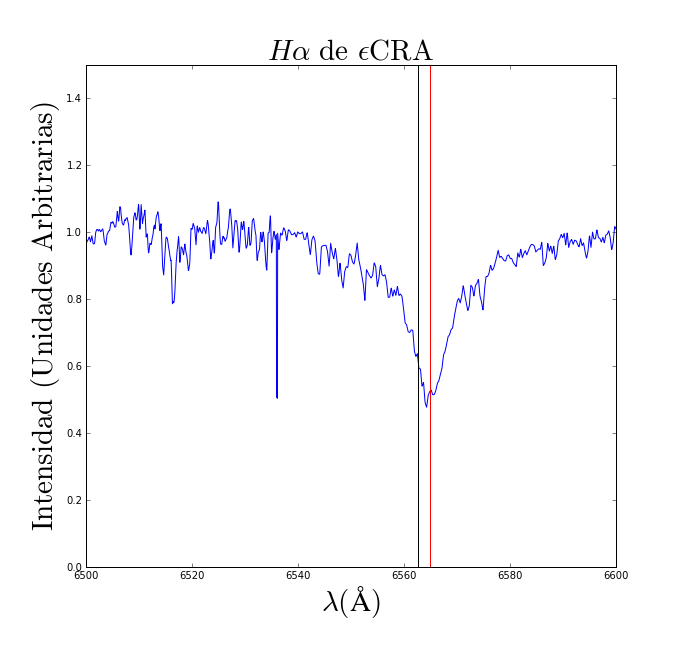
\includegraphics[scale=0.33]{ha2.png}
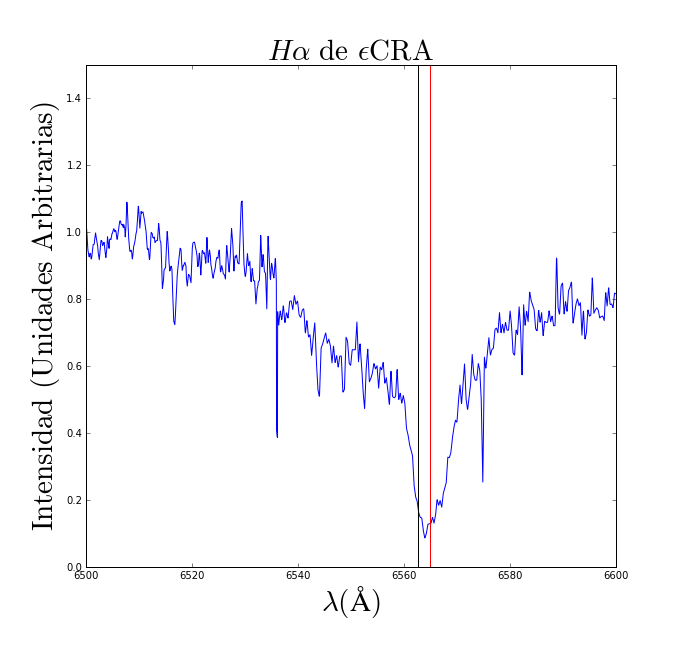
\includegraphics[scale=0.33]{ha3.png}
\caption{Tres diferentes espectros de eps CRA en la region de H$\alpha$\label{ha}}
\end{figure}

Se espera que con al menos 4 espectros mas ya se pueda obtener el periodo de la \'orbita. 
Estos espectros se tomaran en el transcurso del mes de octubre del presente año. 
Todos el tratamiento de los datos se llevo acabo con python y se encuentra disponible en:
https://github.com/jngaravitoc/EpsCra



\section{Referencias}

1. $http://ned.ipac.caltech.edu$  \\
2. Karttunen, Fundamental astronomy 5th edition.\\
3. Alan H. Batten, J. Murray Fletcher and D. G. MacCarthy, http://ad.usno.navy.mil/wds/dsl/SB8/sb8.html\\
4. $http://www.astrosurf.com/buil/isis/isis_en.htm$\\
5. http://www.iau.org/static/public/constellations/gif/CRA.gif \\
6. http://en.wikipedia.org/wiki/File:Schmidt-Cassegrain-Telescope.png \\
7. http://simbad.u-strasbg.fr/simbad/sim-id?Ident=%402353328&Name=V*%20eps%20CrA&submit=submit

\end{document}
